%!TEX encoding = UTF-8 Unicode
% ================================================================================
\documentclass[
    fontsize=12pt,
    headings=small,
    parskip=half,           % Ersetzt manuelles Setzen von parskip/parindent.
    bibliography=totoc,
    numbers=noenddot,       % Entfernt den letzten Punkt der Kapitelnummern.
    open=any,               % Kapitel kann auf jeder Seite beginnen.
%   final                   % Entfernt alle todonotes und den Entwurfstempel.
    ]{scrreprt}
% ===================================Praeambel==================================
\include{stylesvs}
\addbibresource{literaturliste}
% ===================================Dokument===================================

\title{Entwicklung eines Visualisierungswerkzeuges zur Demons-
tration datenschutzfreundlicher Dokumentspeicherdienste}
\author{David Kirchhausen Monteiro}

\begin{document}

\begin{titlepage}% {{{
\includegraphics[width=6.8cm]{../pic/up-uhh-logo-u-2010-u-farbe-u-rgb.pdf}
\begin{center}\Large
	% Universität Hamburg \par
	% Fachbereich Informatik
	\vfill
	Bachelorarbeit
	\vfill
	\makeatletter
	{\Large\textsf{\textbf{\@title}}\par}
	\makeatother
	\vfill
	vorgelegt von
	\par\bigskip
	\makeatletter
	{\@author} \par
	\makeatother
	geb. am 24. Januar 1994 in Hildesheim \par
	Matrikelnummer 6530927 \par
	Studiengang Software-System-Entwicklung
	\vfill
	\makeatletter
	eingereicht am {\@date}
	\makeatother
	\vfill
	Betreuer: Maximilian Blochberger, M. Sc. \par
	Erstgutachter: Prof. Dr.-Ing. Hannes Federrath \par
	Zweitgutachter: Tilmann Stehle, M. Sc.
\end{center}
\ifoptionfinal{}{}
\end{titlepage}% }}}

\chapter*{Aufgabenstellung}
Im  Zuge  dieser  Bachelorarbeit  soll  ein  einfacher  Dokumentenspeicher  entwickelt  werden,
welcher möglichst viele Nutzerdaten erfasst und speichert. Die erfassten Daten sollen anschaulich
grafisch dargestellt werden können. Weiter sollen verschiedene Szenarien entwickelt werden,
welche aufzeigen wie eine mögliche Benutzung des Services mit und ohne der Verwendung
von datenschutzfreundlichen Methoden zum Anonymisieren von Daten aussieht. Anhand der
Szenarien soll eine grafische Auswertung Unterschiede zwischen anonymisierten Daten und
nicht anonymisierten Daten visuell sichtbar machen und die Unterschiede somit leicht zugänglich
sein.

\chapter*{Abstract}
Um ein mögliches Missbrauchspotential und die generelle Informationsgewinnung aus gesammelten Verkehrs- und Metadaten durch Servicebetreiber deutlich zu machen, wird im Rahmen dieser Arbeit ein einfacher Dokumentenspeicher konzipiert und implementiert.
Der Dokumentenspeicher sammelt Verkehrs- und Metadaten und besitzt ein Visualisierungstool um diese gesammelten Daten anschaulich grafisch darzustellen.
Weiter wird ein Szenario definiert und umgesetzt, welches die Benutzung des Dokumentenspeichers exemplarisch aufzeigt.
Die Visualisierungsmöglichkeiten anhand der Beispieldaten des Szenarios vorführt.
Anhand der verschiedenen Visualisierungen wird der potentielle Informationsverlust für einen Servicebetreiber, der durch die Nutzung verschiedener datenschutzfreundlicher Methoden zur Anonymisierung von Daten entsteht, sichtbar gemacht. 

\tableofcontents
\listoffigures
\chapter*{Abkürzungsverzeichnis}
\begin{acronym}[style=nextline]
\acro{API}{Application Programming Interface}
\acro{HTTP}{Hypertext Transfer Protocol}
\acro{HTML}{Hypertext Markup Language}
\acro{d3.js}{Data-Driven Documents Javascript Framework}
\acro{IIS}{Internet Information Service}
\acro{MVC}{Model-view-controller}
\acro{Lat}{Breitengrad (Latitude)}
\acro{Lon}{Längengrad (Longitude)}
\acro{ISP}{Internet Service Provider}
\end{acronym}
\addcontentsline{toc}{chapter}{Abbildungsverzeichnis}

\chapter{Einleitung} \label{Kap:Einleitung}

Dokumentenspeicherdienste sind nützliche Alltagsgegenstände, welche für private sowie kommerzielle Nutzer meist unverzichtbar sind. 
Sie bieten nicht nur den Speicherplatz für wichtige Dateien der Nutzer sondern stellen auch die Sicherheit der Dateien sicher und machen sie global jederzeit verfügbar. 
Durch die große Datensammlung dieser Dienstleister machen sie sich nicht nur selbst zu lukrativen Zielen von gezielten Angriffen (Yahoo, UBER etc.), sondern auch die Dienstleister selber können die Daten auswerten und weitere Metadaten wie z. B. die Dateigröße oder den Autor der Datei sowie Verkehrsdaten wie z. B. die IP-Adresse oder die \ac{HTTP} Header Felder über die Nutzer sammeln und weiterverwenden. 
Vor allem private Nutzer sind meist gar nicht über die Risiken und das Missbrauchspotenzial aufgeklärt, welche die Verwendung solcher Dienstleistungen mit sich bringen. 
Methoden zur Verschlüsselung oder das Anonymisieren von Daten sind Benutzern meist nicht bekannt, werden von den Dienstanbietern nicht angeboten oder sind schwer umzusetzen, da es einen meist erheblichen Aufwand für die Benutzer bedeutet und Kompetenzen erfordert welche diese Benutzer oft nicht besitzen. 
Um genau die Risiken und Missbrauchspotenziale aufzuzeigen wird im Zuge dieser Arbeit ein Dokumentenspeicherdienst entwickelt, welcher Meta- und Verkehrsdaten der Nutzer sammelt und diese in einer visuellen Darstellung zusammenfasst. 
Zur Implementation des Dokumentenspeichers wird dabei das Microsoft ASP.NET Core Framework verwendet. 
Das Framework wird benutzt um die Webbenutzeroberfläche sowie die Web \ac{API} des Dokumentenspeichers zu realisieren. 
Dazu wird das \ac{d3.js}, zur Visualisierung der Daten verwendet. 
Der Dokumentenspeicher soll vor allem den Unterschied zwischen der Verwendung von Methoden zur Verschlüsselung oder das Anonymisieren von Daten visualisieren und verwaltet dazu zwei verschiedene Datensätze, wobei eine Datenmenge ohne, und eine Datenmenge mit der Verwendung von Methoden zur Verschlüsselung oder das Anonymisieren von Daten erzeugt wird. Der entstehende Unterschied der gesammelten Metadaten durch die verschiedenen Methoden führt dann zu einer Veränderung in der Visualisierung, was dann den Effekt und Nutzen der Methoden deutlich sichtbar macht.  
\section{Related Work}
Zu dieser Arbeit werden mehrere Verwandte Arbeiten aufgeführt, welche inhaltlich nah am Thema dieser Arbeit sind.
Die Ergebnisse und Erkenntnisse dieser Arbeiten wurden in dieser Arbeit verwendet um die Aufgabenstellung zu bearbeiten.

[ref- How Unique is your Web Browser] ist ein Artikel in welchem Methoden zum erzeugen eines Fingerprints aus HTTP Headern und Informationen des Browsers beschrieben werden und hinsichtlich ihrer Zuverlässigkeit untersucht werden.
Untersucht wird in wie fern sich ein solcher Nutzerfingerprint eignet um Benutzer daran zuverlässig zu identifizieren.
Als Methoden werden die Auswertung der HTTP Header Felder wie das User-Agent-Feld und das Accept-Feld betrachtet.
Zudem werden mit Hilfe von Javascript weitere Informationen über das System der Benutzer gesammelt.
Diese Methode zum erzeugen eines Fingerprints aus den HTTP Headern für einen Benutzer wird in dieser Arbeit aufgegriffen und verwendet um die Dateien von Benutzern anhand ihres Fingerprints einander korrekt zuzuordnen.
Die Verwendung von Javascript zum Erfassen von weiteten Informationen das Browsers wird dabei nicht verwendet.

[ref - A survey of multiple Tree Visualizations] behandelt verschiedene Mehtoden zur Darstellung von hierarchischen Baumstrukturen.
Dabei werden einzelne, doppelte und multiple Baumstrukturen unterschieden und jeweils mehrere Visualisierungsmethoden aufgeführt.
Für die Visualisierung der im Dokumentenspeicher gesammelten Daten werden im Teil aufgeführte Visualisierungen ausgewählt und implementiert um die Daten anschaulich darzustellen.

\section{Struktur dieser Arbeit}
\todo{Struktur der Arbeit am Ende hier einmal aufführen.}


\chapter{Dokumentenspeicher} \label{Kap:Dokumentenspeicher}

    \section{Verwendungszweck des Dokumentenspeichers} 

Der Dokumenspeicher dient vor allem dazu, die gesammelten Verkehrs- und Metadaten mit und ohne die Verwendung von datenschutzfreundlichen Methoden zum Anonymisieren von Daten, zu vergleichen und deren Unterschiede grafisch möglichst aussagekräftig darzustellen.
Die Unterschiede in den gesammelten Daten sollen zeigen, dass die Verwendung von Methoden zum Anonymisieren von Daten eine Auswirkung darauf hat, ob anhand der gesammelten Verkehrs- und Metadaten, Dateien so einander Zugeordnet werden können, dass die entstehenden Gruppen nur aus den Dateien eines Benutzers entstehen.
%Die Unterschiede in den gesammelten Daten sollen zeigen, dass ohne die Verwendung von Methoden zum Anonymisieren von Daten, Gruppierungen erzeugt werden können, welche der tatsächlichen Anzahl der Benutzer entsprechen.
%Die Verwendung von Methoden zum Anonymisieren hingegen können die Gruppierungen so verändern das die aus den Gruppierungen abgeleitete Anzahl der Benutzer nicht der eigentlichen Anzahl der Benutzer entspricht.
In den Visualisierungen werden deshalb die Dateien anhand verschiedener Eigenschaften ihrer Verkehrs- und Metadaten gruppiert dargestellt.
%Die Unterschiede in den gesammelten Daten sollen zeigen, dass Benutzer anhand ihrer Verkehrs- und Metadaten identifiziert werden können, solange keine datenschutzfreundlichen Methoden zum Anonymisieren der Daten verwendet werden.
%Diese Unterschiede werden in der Visualisierung dadurch sichtbar gemacht, dass Dateien anhand ihrer Verkehrs- und Metadaten gruppiert werden.
Die dabei erzeugten Mengen sind ohne die Verwendung von datenschutzfreundlichen Methoden zum Anonymisieren von Daten bei z. B. der Eigenschaft der IP-Adresse, so eindeutig, dass die dargestellten Mengen den Dateien eines Benutzers entsprechen.
Die Verwendung von datenschutzfreundlichen Methoden zum Anonymisieren von Daten kann jedoch die Identifikation des Benutzers anhand der Verkehrs- und Metadaten verhindern, sodass die erzeugten Mengen in der Visualisierung nicht mehr den tatsächlichen Relationen von Benutzern und Daten entsprechen.

Da für einen Dokumentenspeicher die Verwendung von Authentifizierungen durch einen Benutzeraccount oder ähnliches diese Zuordnung trivialisiert, wird für diesen Dokumentenspeicher eine solche Authentifizierung nicht verwendet.
Für diesen Dokumentenspeicher wird zudem angenommen, dass alle Dateien von den Benutzern so verschlüsselt wurden, dass nur die Benutzer in der Lage sind, sie wieder zu entschlüsseln.
Daher werden alle Dateien durch kryptografische Methoden logisch getrennt in einen gemeinsamen Speicher abgelegt.
\todo{mandantenspezifische Verschlüsselung, siehe ...}

Um die Effekte einer datenschutzfreundlichen Methode zur Anonymisierung von Daten aufzeigen zu können, müssen die gesammelten Dateien im Dokumentenspeicher unterscheidbar sein in Daten mit und ohne Anonymisierung. 
Dies wird durch die Verwendung zweier API-Endpunkte erreicht, die beim Hochladen der Dateien durch die Benutzer zu wählen sind.
Im Dokumentenspeicher gibt es also eine Datenmenge von Dateien, welche durch die Nutzung von datenschutzfreundlichen Methoden zum Anonymisieren geschützt sind und eine ungeschützte Datenmenge.
Damit diese Datenmenge vergleichbar sind sieht die Verwendung des Dokumentenspeichers vor das für den Vergleich von geschützten und ungeschützten Datenmengen die zu untersuchenden Daten einmal mit und ohne die Verwendung von Methoden zum Anonymisieren von Daten hochgeladen werden. 
Dabei sollte möglichst darauf geachtet werden das die so entstehenden Datenmengen sich nur durch die Verwendeten Methoden zum Anonymisieren der Daten unterscheiden. 
Die daraus resultierenden Datenmengen eignen sich dazu einmal die Visualisierung der ungeschützten Datenmenge zu zeigen und die daraus ableitbaren Informationen visuell sichtbar zu machen.
Die geschützte Menge sollte dann im Kontrast dazu sichtbar machen das durch die Verwendete Methode zum Anonymisieren von Daten die abgeleiteten Informationen nicht mehr in allen Aspekten denen der ungeschützten Datenmenge entsprechen.
Ein entsprechendes Szenario, welches diese Verwendung exemplarisch darstellt ist in Kapitel~\ref{AliceBob} zu sehen.
Alternativ ist es jedoch auch möglich Datenmengen aus geschützten und ungeschützten Daten zu betrachten.
Dafür sollten alle Dateien an einen \ac{API}-Endpunkt gesendet werden, sodass alle Dateien in der selben Datenmenge vorhanden sind.
Die Betrachtung von einer solchen gemischten Datenmenge aus geschützten und ungeschützten Daten kann ebenfalls benutzt werden um den Effekt von verschieden Methoden zum Anonymisieren von Daten aufzuzeigen, kann aber nicht aufzeigen wie die gleiche Datenmenge unterschiedlich ausgewertet werden kann und somit unterschiedliche Visualisierungen entstehen, abhängig davon ob und welche Methoden zum Anonymisieren der Daten verwendet wurde. 

In dem Visualisierungstool des Dokumentenspeichers kann eine Visualiserung ausgewählt werden und beliebig zwischen der geschützten Datenmenge und der ungeschützten Datenmenge gewechselt werden, sodass die Unterschiede anhand der Visualisierung der beiden Datenmengen leicht erkennbar sind.
Der Dokumentenspeicher kann aber auch zur Visualisierung von einer gemischten Datenmenge aus geschützten und ungeschützten Dateien verwendet werden. 
Dies wird erreicht, indem die ungeschützten und geschützten Dateien lediglich über einen \ac{API}-Endpunkt hochgeladen werden.

Die Verwendung reiner Datenmengen (aus nur ungeschützten und nur geschützten Dateien) eignet sich somit, die entstehenden Unterschiede durch die Verwendung von datenschutzfreundlichen Methoden zum Anonymisieren von Daten und ohne diese zu Visualisieren und somit ausschließlich diese Unterschiede zu Visualisieren, da die zugrunde liegenden Dateien sich sonst nicht unterscheiden. 

    \section{Implementation des Dokumentenspeichers}    
    
    \subsection{Verwendete Technologien}
Der Dokumentenspeicher wurde mit Hilfe des ASP.NET Core Framework erstellt. 
Das Framework ist Microsofts aktuellstes plattformübergreifendes Framework zur Realisierung von Webanwendungen.
Das Framework unterstützt alle gängigen Betriebssysteme wie Windows, Mac OS und Linux.
Mit dem ASP.NET Core entwickelte Webanwendungen lassen sich in gängige Hostingplattformen, wie z. B. der \ac{IIS} von Microsoft, integrieren oder können auch in einem eigenen Prozess selbst gehostet werden. 
Das ASP.NET Core Framework sieht dabei eine \ac{MVC} Architektur der Projekte vor und verwenden diese Architektur intern zum Realisieren der Anwendungen. 
Als Model wird in diesem Kontext ein Objekt zur Datenrepräsentation verstanden. 
Ein View ist eine HTML-Seite, die an den Klienten ausgegeben wird. Controller sind die zentralen Elemente mit verschiedenen Funktionen. 
Sie stellen die Funktionalität von Views auf der Serverseite sicher.
Sie sind zur Steuerung verschiedener Routen und die Implementation von \ac{API}-Endpunkten vorgesehen und verwalten dabei die zugrunde liegenden Datenbanken.

\newpage
    \subsection{Aufbau des Dokumentenspeichers}

Der entwickelte Dokumentenspeicher besteht aus
\begin{itemize}
\item einer Model-Klasse,
\item drei View-Klassen,
\item einer Controller-Klasse, sowie
\item einer Datenbankkontext-Klasse.
\end{itemize}

Die Model-Klasse hält für alle erfassten Verkehrs- und Metadaten Eigenschaften bereit, welche diese repräsentieren.

\begin{description}[style=nextline]
\item[ID] Datenbank Index
\item[Set] Gruppe, welcher die Datei zugeordnet wurde (geschützte oder ungeschützte Gruppe)
\item[Filename] Dateiname
\item[Filepath] Pfad zur gespeicherten temporären Datei
\item[Size] Dateigröße in Byte
\item[IPAddress]  IP-Adresse von der die Datei hochgeladen wurde
\item[Headers] String bestehend aus den Headern der Datei
\item[HeaderFingerprint] Hash erzeugt aus dem Zusammenschluss von ausgewählten Headerfeldern
\item[DateTime] Zeitstempel für das Hochladen der Datei
\item[Country] Land aus welchem die Datei hochgeladen wurde
\item[RegionName] Region (Bundesland) aus welchem die Datei hochgeladen wurde
\item[City] Stadt aus welchem die Datei hochgeladen wurde
\item[Lat] Breitengrad welcher mit der bekannten IP-Adresse assoziiert wird
\item[Lon] Längengrad welcher mit der bekannten IP-Adresse assoziiert wird
\item[ISP] Der Internetanbieter welcher der IP zugeordnet ist
\end{description}

Mit Hilfe der Model-Klasse werden die gesammelten Daten sowie der fad zu der gespeicherten Datei in der Datenbank abgelegt.

Die drei View-Klassen repräsentieren die HTML-Seiten, welche von einem Benutzer über bestimmte Routen aufgerufen werden können:
\begin{description}[style=nextline] 
\item[/FileEntry] Anzeige der Datenbank in tabellarischer Form
\item[/FileEntryCreate] Bietet Möglichkeiten zum Hochladen von Dateien oder dem Erzeugen von Pseudodaten
\item[/FileEntryVisual] Visualisierung der gesammelten Daten
\end{description}

Die \text{FileEntry} HTML-Seite ist die Startseite der Webanwendung und verweist zu der \textit{FileEntryCreate} und \textit{FileEntryVisual}.
Zudem zeigt sie die Datenbank in tabellarischer Form getrennt in die beiden möglichen Gruppen durch die verschiedenen \ac{API}-Endpunkten.
Diese Seite ist hauptsächlich zur Entwicklung gebraucht worden.
Die \textit{FileEntryCreat} HTML-Seite enthält mehrere Funktionen um Dateien hochzuladen.
Dabei können die jeweils verschiedenen \ac{API}-Endpunkte ausgewählt werden oder Beispieldaten über verschiedene Text eingaben erzeugt werden. 
Diese Seite ist ebenfalls hauptsächlich zur Entwicklung des Dokumentenspeichers verwendet worden.
Die \textit{FileEntryVisual} HTML-Seite bietet verschiedene Visualisierungsmögichkeiten an und ist der Hauptbestandteil des Dokumentenspeichers.

Die Controller-Klasse implementiert verschiedene \ac{API}-Endpunkte, welche das Hochladen von Dateien und die Abfrage der gesammelten Daten ermöglicht.
\begin{description}[style=nextline]   
\item[/api/GetA] \ac{HTTP} Get Methode welche die gesammelten Verkehrs- und Metadaten der ungeschützten Daten ausgiebt
\item[/api/GetB] \ac{HTTP} Get Methode welche die gesammelten Verkehrs- und Metadaten der geschützten Datensatz ausgiebt
\item[/api/uploadA] \ac{HTTP} Post Methode zum hochladen von ungeschützten Dateien
\item[/api/uploadB] \ac{HTTP} Post Methode zum hochladen von geschützten Dateien
\item[api/uploadEmu] \ac{HTTP} Post Methode zum erzeugen von Dummydaten
\item[api/getFile] \ac{HTTP} Get Methode zum herunterladen einer Datei
\end{description}

Beim Hochladen der Dateien werden in der Controller-Klasse die Verkehrs- und Metadaten der Dateien erfasst, sowie die hochgeladenen Dateien abgespeichert.
Während die einige Eigenschaften direkt aus den Verkehrs- und Metadaten entnommen werden können, werden andere Eigenschaften durch die Auswertung oder Weiterverwendung  der Verkehrs- und Metadaten erzeugt.
Der Headerfingerprint wird so aus dem Zusammenschluss aus dem Header-Feldern:
\begin{itemize}
\item User-Agent
\item Accept
\item Accept-Encoding
\end{itemize}
erzeugt.
Die Kombination dieser Werte wird gehasht und als Headerfingerprint gespeichert.

Die Datenbankkontext-Klasse dient der Verwaltung und dem Zugriff auf die Datenbank.

Für die Visualisierung ist es wesentlich, zwischen den einzelnen Visualisierungen wechseln zu können.
Daher besteht die \textit{FileEntryVisual} \ac{HTML}-Seite aus neben einem Bereich für die Darstellung der Visualisierung auch aus einem Navigationsbereich.
Die Navigation bietet die Möglichkeit zwischen den ungeschützten und geschützten Datensatz zu wechseln, verschiedene Visualisierungsmöglichkeiten auszuwählen und hat einen Bereich wo die gesammelten Verkehrs- und Metadaten einer ausgewählten Datei aufgelistet werden können.
Implementiert sind drei Visualisierungsmöglichkeiten:
\begin{itemize}
\item eine Baumkarte (Treemap)
\item eine geografische Karte mit der Anzeige von Standpunkten und
\item einem Zeitstrahl
\end{itemize} 

\textit{Baumkarte}: Eine Baumkarte ist eine Möglichkeit eine Baumstruktur darzustellen, wobei Boxen entsprechend der Baumstruktur in einander geschachtelt werden\footnote{\url{https://datavizcatalogue.com/methods/treemap.html}}. 
Bei der Verwendung der Baumkarte muss eine Eigenschaft der Model-Klasse (ausgenommen \textit{Filepath}) ausgewählt werden um eine Baumstruktur zu bilden.
Diese ausgewählte Eigenschaft wird als Schlüsseleigenschaft für die Baumkarte bezeichnet und ist die Eigenschaft der gesammelten Verkehrs- und Metadaten nachdem gruppiert werden soll.
Die Baumstruktur besteht aus einem Wurzelknoten, den davon abgehenden Kindknoren und den von diesen abgehenden Blattknoten, welche sich dadurch auszeichnen, dass von ihnen keine weiteren Knoten Abgehen.
Der Wurzelknoten wird über die Schlüsseleigenschaft erzeugt.
Die restlichen Knoten werden aus den gegebenen Daten erzeugt, sodass alle Dateien mit der gleichen Eigenschaft für die gewählte Schlüsseleigenschaft unter einem Knoten zusammen gefasst werden.
Die Knoten dieser Eigenschaften werden unter dem Wurzelknoten angeordnet.
Die erzeugt Baumstruktur hat somit drei Ebenen.
Auf der 1. Ebene den Wurzelknoten mit der gewählten Schlüsseleigenschaft.
Auf der 2. Ebene die Knoten welche die gesammelten Werte für diese Schlüsseleigenschaft darstellen.
Auf der 3. Ebene die Dateien, welche entsprechend ihres Wertes im Bezug auf die Schlüsseleigenschaft dem entsprechenden Knoten der 2. Ebene untergeordnet wurden.

Abbildung~\ref{fig:baum} zeigt eine Beispielhafte Baumstruktur für sechs Dateien, die über zwei verschiedene IP-Adressen hochgeladen wurden. 
Der Wurzelknoten zeigt die Schlüsseleigenschaft: \textit{IP-Adresse}.
Auf der 2. Ebene werden die gesammelten IP-Adressen angezeigt.
Auf der 3. Ebene werden die Dateien den jeweiligen IP-Adressen zugeordet.
In dieser Abbildung die Dateien data0, data1 und data2 zu der IP-Adresse 192.0.2.1 und data3, data4 und data5 zu der IP-Adresse 192.0.2.2.

\begin{figure}[H]
\centering
	\begin{forest}
  	for tree={%
    	folder,
    	grow'=0,
    	fit=band,
  	}
  	[Schlüsseleigenschaft: IP-Adresse
  		[192.0.2.1
			[data0]
			[data1]
			[data2]  		
  		]
  		[192.0.2.2
			[data3]  	
  			[data4]
  			[data5]
  		]
  	]
	\end{forest}
\caption{Beispielhafte Baumstruktur für das erstellen einer Baumkarte}
\label{fig:baum}
\end{figure}

Aus dieser Struktur wird nun die Baumkarte erzeugt. Für jeden Knoten im Baum wird eine Box erzeugt, dabei wird jeder untergeordneter Knoten in die Box des übergeordneten Knotens eingebettet und in Abhängigkeit zu diesem eingefärbt.
Durch diese farblichen Unterschiede sollen dann die verschiedenen Ebenen und Relationen deutlich werden.
Eine Schematische Darstellung des Beispiels ist in Abbildung~\ref{fig:schem} zu sehen.

\begin{figure}[H]
\centering
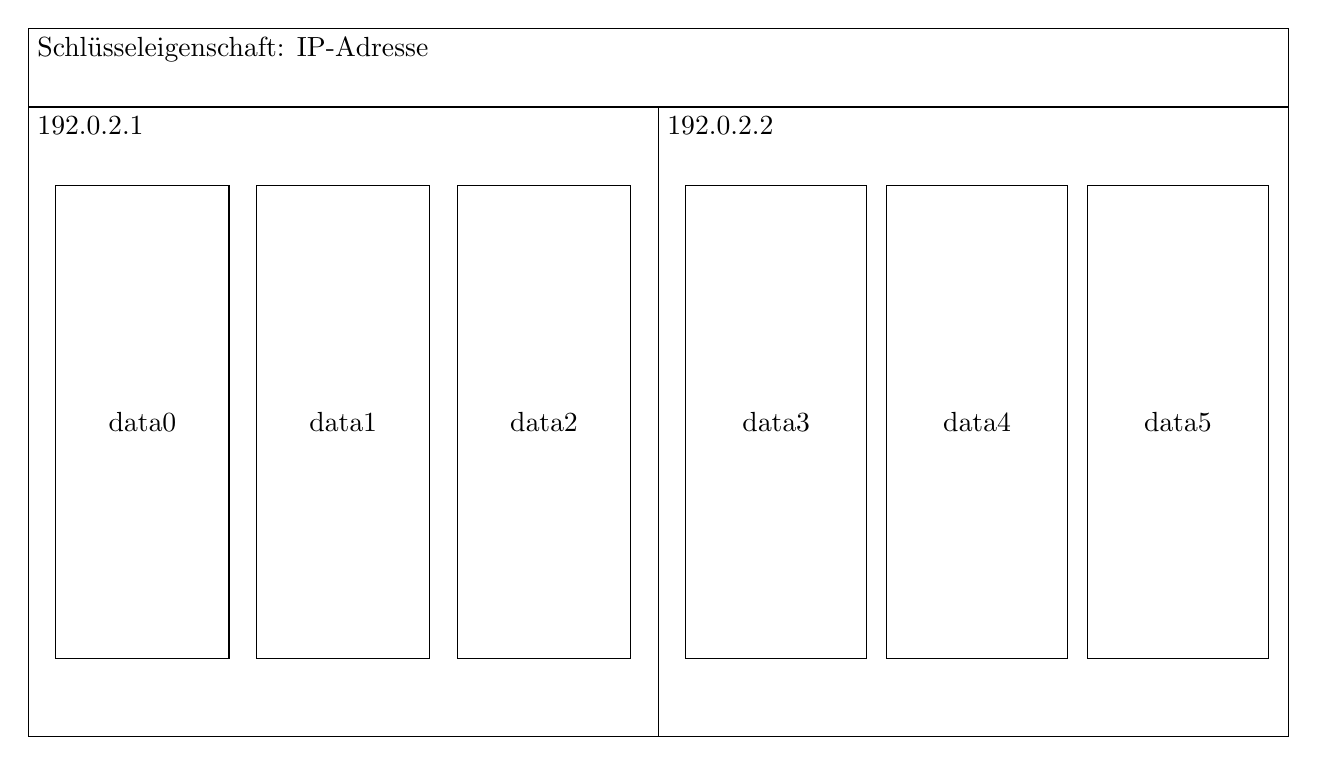
\begin{tikzpicture}
\node (rect) [rectangle, draw, minimum width=160mm, minimum height=90mm, anchor= north west] at (0,0) {};
\node [below right] at (rect.north west) {Schlüsseleigenschaft: IP-Adresse};

\node (rectA) [rectangle, draw, minimum width=80mm, minimum height=80mm, anchor= north west] at (0,-1) {};
\node [below right] at (rectA.north west) {192.0.2.1};

\node (rectA0) [rectangle, draw, minimum width=22mm, minimum height=60mm, anchor= north west] at (0.35,-2) {};
\node [] at (rectA0.center) {data0};
\node (rectA1) [rectangle, draw, minimum width=22mm, minimum height=60mm, anchor= north west] at (2.9,-2) {};
\node [] at (rectA1.center) {data1};
\node (rectA2) [rectangle, draw, minimum width=22mm, minimum height=60mm, anchor= north west] at (5.45,-2) {};
\node [] at (rectA2.center) {data2};

\node (rectB) [rectangle, draw, minimum width=80mm, minimum height=80mm, anchor= north west] at (8,-1) {};
\node [below right] at (rectB.north west) {192.0.2.2};

\node (rectB0) [rectangle, draw, minimum width=23mm, minimum height=60mm, anchor= north west] at (8.35,-2) {};
\node [] at (rectB0.center) {data3};
\node (rectB1) [rectangle, draw, minimum width=23mm, minimum height=60mm, anchor= north west] at (10.9,-2) {};
\node [] at (rectB1.center) {data4};
\node (rectB2) [rectangle, draw, minimum width=23mm, minimum height=60mm, anchor= north west] at (13.45,-2) {};
\node [] at (rectB2.center) {data5};
\end{tikzpicture}
\caption{Schematische Darstellung der Visualisierungsmöglichkeiten der Baumstruktur}
\label{fig:schem}
\end{figure}

\textit{geografische Karte}: Die Verwendung der Darstellung der Dateien als Standpunkte auf einer Karte basiert auf den Eigenschaften Breitengrad (Latitude) und Längengrad (Longitude) der Model-Klasse.
Für die Bestimmung eines Standpunktes anhand der IP-Adresse wird die \ac{API} von \url{http://ip-api.com} verwendet.
Von der \ac{API} werden die Längen- und Breitengrade, sowie die Information zu Land, Region, Stadt und des Internetanbieters abgefragt.
Die Längen- und Breitengrade werden zur Darstellung der Standpunkte auf der Karte verwendet. 

\textit{Zeitstrahl}: Die Darstellung als Zeitstrahl zeigt, wie viele Dateien zu einen Zeitpunkt hochgeladen wurden.
Die X-Achse repräsentiert die Zeit und die Y-Achse die Anzahl der Dateien.

In Abbildung~\ref{fig:VisualPageAll} ist eine beispielhafte \textit{FileEntryVisual} \ac{HTML}-Seite zu sehen.
Die \ac{HTML}-Seite wird eine Baumkarte dargestellt im rechten Teil des Fensters dargestellt.
Die repräsentierten Daten beziehen sich auf die im Szenario des Kapitel~\ref{Kap:Szenarios} Beispieldaten und werden dort näher beschrieben.
Im linken Bereich des Fensters ist der Navigationsbereich zu erkennen.
Es wird das ausgewählte \textit{Set A} angezeigt, welches die ungeschützten Daten repräsentiert.
Für das Wechseln zwischen den beiden Datenmengen \textit{Set A} und \textit{Set B} sind zwei Schaltflächen mit den Beschreibungen A und B zu erkennen.
Unter den beiden Schaltflächen sind zwei Auswahlmenüs platziert. 
Das obere zur Auswahl der Visualisierungsmethode, das Untere zur Auswahl der Schlüsseleigenschaft, welche zum Erstellen der Baumkarte benötigt wird.
Darunter sind die verschiedenen Eigenschaften für eine ausgewählte Datei aufgelistet.
Die ausgewählte Datei in der Abbildung ist dataAlice1, welche in der Visualisierung im rechten Teil des Fensters als grüne Box zu erknnen ist.
Durch das Anklicken der Box werden die Eigenschaften dieser Datei angezeigt.
\begin{figure}[H]
\includegraphics[width=0.7\textwidth]{../pic/VisualPageAll.png}
\captionof{figure}{FileEntryVisual HTML-Seite mit Beispieldaten aus Kapitel~\ref{Kap:Szenarios}}
\label{fig:VisualPageAll}
\end{figure}

\chapter{Szenario} \label{Kap:Szenarios}

Um die Visualisierungen erzeugen zu können werden Daten benötigt, die verschiedenen Benutzern gehören.
Diese Daten sollen wie bereits ausgeführt als geschützte Daten und ungeschützte Daten vorhanden sein. 
Dafür wird im folgenden ein Szenario definiert, anhand welchem die Visualisierungen beispielhaft dargestellt werden. 
Dieses Beispiel basiert nicht auf echt Daten.
Die Daten wurden so gewählt, dass der Effekt der Visualisierung präsentiert werden kann.
%Dieses Beispiel ist hypothetisch und es gibt keine zugrunde liegenden Daten. 
Die Verkehrs- und Metadaten werden für jeden Benutzer so gewählt, dass diese sich unterscheiden. 
Für die genauen Daten werden Standartwerte und Beispieledaten aus anderen Quellen verwendet. 

    \section{Beispiel: Alice und Bob} \label{AliceBob}
Um die Visualisierungen an einem Beispiel zu erläutern wird ein Szenario definiert, welches die Benutzung des Dokumentenspeichers und die verwendeten Daten beschreibt.
Dazu werden zwei Benutzer Alice und Bob definiert, welche sich beide in Hamburg befinden und sich in den Verkehrs- und Metadaten unterscheiden, sodass sie anhand dieser klar unterschieden werden können.
Alice und Bob laden jeweils drei Dateien mit und ohne die Verwendung einer Methode zum Anonymisieren ihrer Daten hoch.
Alice Dateien sind dataAlice1, dataAlice2 und dataAlice3 und Bobs Dateien sind dataBob1, dataBob2 und dataBob3 und haben alle unterschiedliche Dateigrößen.
Die Verkehrs- und Metadaten für diese Dateien sind so gewählt, dass sie sich die Verkehrsdaten von Alice und Bob im \textit{User-Agent} Headerfeld unterscheiden und jede Datei eine andere Größe besitzt.
Es wird angenommen, dass die Dateien von Alice einzeln in einem Abstand von mindestens zehn Minuten hochgeladen werden.
Die Dateien von Bob werden alle zusammen in einem Dateiupload hochgeladen.
Für die Verwendung einer Methode zum Anonymisieren ihrer Daten werden zwei Fälle betrachtet:
\begin{enumerate}
\item Die Verwendung eines Proxys, welcher von Alice und Bob verwendet wird.
\item Die Verwendung des Tor-Netzwerks von Alice und Bob.
\end{enumerate}
Für den Proxy nehmen wir an das die End-to-End Header korrekt übermittelt werden.
Bei der Verwendung des Tor-Netzwerks nehmen wir an das Alice und Bob den Tor-Browser verwenden und die Standarteinstellungen des Browsers nicht verändert haben.

Die zu visualisierenden Daten bestehen dem nach aus drei Datenmengen:
\begin{itemize}
\item der ungeschützten Datenmenge
\item der durch einen Proxy geschützten Datenmenge
\item und der durch die Verwendung der Tor-Netzwerks geschützten Datenmenge.
\end{itemize}
Die Visualisierungen dieser drei Datenmengen werden in den folgenden Abschnitten vorgestellt und ausgewertet.

Für die Benutzer nehmen wir folgende Verkehrs- und Metadaten an: 
\paragraph{Alice}
\begin{itemize}
  \item IP: 
  \begin{itemize}
  \item IP-Adresse: 192.0.2.1
  \item \ac{Lat}: 53.5770988464355 \ac{Lon}: 10.0190000534058
  \item Land: Deutschland Region: Hamburg Stadt: Hamburg
  \end{itemize}
  \item Headerfingerprint: \textit{db9080...} aus :
  \begin{itemize}
  \item \textit{Accept}: text/html, application/xhtml+xml, application/xml;q=0.9,*/*;q=0.8s
  \item \textit{Accept-Encoding}: gzip, deflate
  \item \textit{User-Agent}: Mozilla/5.0 (Macintosh; Intel Mac OS X 10\_11\_6) AppleWebKit/601.7.7 (KHTML, like Gecko) Version/9.1.2 Safari/601.7.7
  \end{itemize}
\end{itemize}

\paragraph{Bob}
\begin{itemize}
  \item IP: 
  \begin{itemize}
  \item IP-Adresse: 192.0.2.2
  \item \ac{Lat}: 53.5830001831055 \ac{Lon}: 9.98130035400391
  \item Land: Deutschland Region: Hamburg Stadt: Hamburg
  \end{itemize}
  \item Headerfingerprint: \textit{438eda...} aus:
  \begin{itemize}
  \item \textit{Accept}: text/html, application/xhtml+xml, application/xml;q=0.9,*/*;q=0.8
  \item \textit{Accept-Encoding}: gzip, deflate
  \item \textit{User-Agent}: Mozilla/5.0 (Windows NT 10.0; Win64; x64; rv:60.0) Gecko/20100101 Firefox/60.0
  \end{itemize}
\end{itemize}

Alice und Bob unterscheiden sich so anhand der Relevanten Header-Felder für die Erzeungung des Headerfingerprints nur in dem \textit{User-Agent}-Feld.

\section{IP-Adressen bezogene Visualisierung} \label{ipVis}

In den weiteren Abbildungen dieses Kapitels werden immer die Beispieldaten von Alice und Bob mit dem Visualisierungstool des Dokumentenspeichers dargestellt.

Die Abbildung~\ref{fig:ungIpTM} zeigt die Visualisierung der Baumkarte für die Datenmenge der ungeschützten Dateien nach dem schematischem Beispiel aus Abbildung~\ref{fig:schem}. 
In Abbildung~\ref{fig:ungIpTM} ist eine blauer Box als Wurzelknoten zu erkennen, welche den Titel: \glqq \textit{Key: ipAddress}\grqq ~trägt und damit die damit die gewählte Schlüsseleigenschaft benennt.
In diese Box sind zwei orange Boxen eingebettet.
Beide Kästen tragen einen Titel, der obere \glqq \textit{Key: 192.0.2.1}\grqq, die IP-Adresse von Alice, und der untere \glqq \textit{Key: 192.0.2.2}\grqq, die IP-Adresse von Bob.
In den oberen Box (mit Alices IP-Adresse betitelt) sind drei weitere grüne Boxen eingebettet, welche für die Dateien dataAlice1, dataAlice2 und dataAlice3 stehen.
In der unteren Box (mit Bobs IP-Adresse betitelt) sind drei rote Boxen eingebettet, welche die Dateien dataBob1, dataBob2 und dataBob3 darstellen.
Die Farbe der einzelnen Boxen ist anhängig von dem jeweiligen Elternknoten in der Baumstruktur, sodass Kindknoten eines Knoten immer gleich eingefärbt sind.
Somit wird die Zusammengehörigkeit von Dateien anhand der farblichen Markierung sofort sichtbar.
Die blaue Box stellt immer den Wurzelknoten dar, die orangenen dessen Kindknoten, welche die Einträge für die gewählte Schlüsseleigenschaft der gesammelten Verkehrs- und Metadaten sind.
Hier in diesem Beispiel die IP-Adressen von Alice und Bob.

In Abbildung~\ref{fig:ungIpM} ist eine Karte von Hamburg Zentrum zu erkennen.
Auf dieser Karte sind 2 Standpunkte markiert.
Ein Punkt bei \ac{Lat}: 53.5770988464355 \ac{Lon}: 10.0190000534058, welcher aus der IP-Adresse von Alice ermittelt wurde und dem definierten Standpunkt von Alice entspricht.
Der zweite Punkt liegt bei \ac{Lat}: 53.5830001831055 \ac{Lon}: 9.98130035400391, welcher aus der IP-Adresse von Bob ermittelt wurde und definierten Standpunkt von Bob entspricht.
Beim Überfliegen eines Punktes mit der Maus wird für jeden Punkt die zugehörige IP-Adresse als Tooltip\footnote{siehe \url{https://en.wikipedia.org/wiki/Tooltip}} angezeigt und die Anzahl von Dateien, welche von dieser IP-Adresse hochgeladen wurden.

\begin{figure}[H]
\includegraphics[width=0.7\textwidth]{../pic/vec/IP-Proxy-SetA-tree3.png}
\captionof{figure}{Baumkarte der IP-Adressen der ungeschützten Beispieldaten von Alice und Bob}
\label{fig:ungIpTM}
\end{figure}

\begin{figure}[H]
\includegraphics[width=0.5\textwidth , height=0.4\textheight]{../pic/IP-Proxy-SetA.PNG}
\captionof{figure}{Standorte ermittelt aus den ungeschützten Beispieldaten von Alice und Bob}
\label{fig:ungIpM}
\end{figure}

Die Darstellung der Daten spiegelt somit die definierten Beispieldaten korrekt wieder und erlaubt es die jeweiligen Daten den richtigen Benutzer zuzuordnen. 
Der Servicebetreiber kennt somit die Position von Alice und Bob und kann die von ihnen hochgeladenen Dateien durch die IP-Adresse identifizieren.

Für die Verwendung von datenschutzfreundlichen Methoden zum Anonymisieren von Daten ergeben sich de folgenden Abbildungen.

Beim Betrachten des ersten Falls, der Verwendung eines Proxys, ergeben sich die Visualisierung wie in Abbildung~\ref{fig:PIpTM} und Abbildung~\ref{fig:PIpM}.
In Abbildung~\ref{fig:PIpTM} ist nur eine orangener Box für die IP-Adresse des Proxys dargestellt.
Alle sechs definierten Dateien, die Dateien von Alice dataAlice1, dataAlice2 und dataAlice3 und die Dateien von Bob dataBob1, dataBob2 und dataBob3, sind dieser IP-Adresse zugeordnet und als grüne Boxen unter der IP-Adresse des Proxys angeordnet.
In Abbildung~\ref{fig:PIpM} ist ein Standpunkt in Berlin markiert.
Der Standpunkt liegt bei \ac{Lat}: 52.5167 \ac{Lon}: 13.4 und ist durch die IP-Adresse des Proxys ermittelt worden. 

\begin{figure}[H]
\includegraphics[width=0.7\textwidth]{../pic/IP-Proxy-SetB-tree3.PNG}
\captionof{figure}{Baumkarte der IP-Adresse der Beispieldaten von Alice und Bob bei der Verwendung eines Proxys}
\label{fig:PIpTM}
\end{figure}

\begin{figure}[H]
\includegraphics[width=0.5\textwidth , height=0.2\textheight]{../pic/IP-Proxy-SetB.PNG}
\captionof{figure}{Standorte von Alice und Bob bei der Verwendung eines Proxys}
\label{fig:PIpM}
\end{figure}

Beim Vergelich der Abbildung\ref{fig:ungIpTM} und \ref{fig:PIpTM} sowie \ref{fig:ungIpM} und \ref{fig:PIpM} ist klar zu erkennen, dass durch die Verwendung eines Proxys, der Servicebetreiber die einzelnen Dateien nicht mehr anhand der IP-Adresse deren tatsächlichen Besitzern zugeordnet werden kann.
Die Zuordnung der Dateien zu einer einzelnen IP-Adresse lässt dem Servicebetreiber bei der alleinigen Betrachtung der IP-Adresse nur darauf schließen das alle Dateien von dem selben Benutzer stammen.
Die Dateien von Alice und Bob sind somit durch die Verwendung des Proxys durch eine Anonymitätsmenge geschützt, sodass die Dateien in der durch die IP-Adresse erzeugte Gruppierung anonym werden.
Da die Beispieldaten zwei Benutzer definieren und der Servicebetreiber anhand des verwendeten Proxys nur auf einen Benutzer schließen kann ist der Effekt durch die Verwendung des Proxys klar anschaulich geworden. 

Abbildung~\ref{fig:TIpTM} und \ref{fig:TIpM} zeigen die Visualisierungen für die Verwendung des Tor-Netzwerks als Methode zum Anonymisieren der Daten.
In der Abbilung~\ref{fig:TIpTM} sind vier verschiedene orange Boxen für vier verschiedene IP-Adressen abgebildet.

Die Zuordnung der Dateien zu den IP-Adressen entspricht:
\begin{description}[style=nextline]
%\centering
\item[203.0.113.1] Datei: dataAlice1, Farbe: grün
\item[203.113.5] Datei: dataAlice2, Farbe: lila
\item[203.0.113.13] Datei: dataAlice3, Farbe: braun
\item[203.0.113.2] Farbe: rot
\begin{enumerate}
\item dataBob1
\item dataBob2
\item dataBob3
\end{enumerate}
\end{description}

Für jede dieser IP-Adressen ist in der Karte in Abbildung~\ref{fig:TIpM} ein Standort abgebildet, welche über Deutschland verteilt sind. 
\begin{description}
\item[1] Naumburg - \ac{Lat}:50.8919 \ac{Lon}:11.8682
\item[2] Karlsruhe (Innenstadt-Ost) - \ac{Lat}:49.0096 \ac{Lon}:8.41217
\item[3] Frankfurt am Main - \ac{Lat}:50.1109 \ac{Lon}:8.68213
\item[4] Berlin (Charlottenburg-Wilmersdorf) - \ac{Lat}:52.5239 \ac{Lon}:13.3214
\end{description}

\begin{figure}[H]
\includegraphics[width=0.7\textwidth]{../pic/IP-Tor-SetB-tree4.png}
\captionof{figure}{Baumkarte der IP-Adresse der Beispieldaten von Alice und Bob bei der Verwendung des Tor-Netzwerks}
\label{fig:TIpTM}
\end{figure}

\begin{figure}[H]
\includegraphics[width=0.4\textwidth]{../pic/IP-Tor-SetB-Map.png}
\captionof{figure}{Standorte der Dateien von Alice und Bob bei der Verwendung des Tor-Netzwerks}
\label{fig:TIpM}
\end{figure}

Vergleicht man wiederum Abbildung~\ref{fig:ungIpTM} mit \ref{fig:TIpTM} und \ref{fig:ungIpM} mit \ref{fig:TIpM} fallen deutliche Unterschiede der Visualisierungen auf. 
Während wie bereits (oben) ausgeführt in Abbildung~\ref{fig:ungIpTM} die Beispieldaten korrekt gruppiert visuell dargestellt werden,
lässt die Darstellung aus Abbildung~\ref{fig:TIpTM} und Abbildung~\ref{fig:TIpM} dies nicht mehr zu.
Die Dateien von Bob können zwar zusammen geordnet werden, jedoch sind die Dateien von Alice auf drei verschiedene IP-Adressen verteilt.
Die Gruppierung der Dateien von Bob ist zwar korrekt jedoch entspricht die IP-Adresse und somit auch der Standort der daraus abgeleitet ist nicht mehr dem eigentlichen Beispiel und ist darauf zurück zu führen, dass die Dateien alle zusammen hochgeladen wurden.
Ein Servicebetreiber muss so anhand der IP-Adresse annehmen, dass die Dateien von vier verschiedenen Benutzern stammen.
Dies widerspricht klar den definierten Daten und zeigt die Anonymisierung der Daten durch die Verwendung des Tor-Netzwerks.

Die Betrachtung beider Fälle von Anonymisierung (Verwendung eines Proxys oder des Tor-Netzwerks) ergibt, das beide Schutzmethoden im Hinblick auf die IP-Adresse einen derart ausreichenden Effekt gehabt haben, dass eine korrekte Zuordnung von Datei und Benutzer bezüglich der IP-Adresse nicht mehr möglich waren.

\section{Headerfingerprint bezogene Visualisierung}
Nach der Auswertung der Informationen, welche aus der IP-Adressbezogenen Visualisierung abgeleitet werden können.
Kann ein Servicebetreiber weitere der gesammelten Eigenschaften untersuchen um festzustellen ob andere Eigenschaften die gleichen Schlussfolgerungen erlauben wie die IP-Adresse und diese somit erhärten oder ob andere Eigenschaften zu anderen Schlussfolgerungen führen.

Um die Veränderungen bezüglich des Headerfngerprints visualisieren zu können, muss in der \textit{FileEntryVisual} \ac{HTML}-Seite im Navigationsbereich die Schlüsseleigenschaft auf den \textit{headerFingerprint} umgestellt werden.

Für die ungeschützten Beispieldaten von Alice und Bob erhalten wir die Visualisierung als Baumkarte, wie sie in  Abbildung~\ref{fig:ungHTM} gezeigt wird.
Zuerkennen sind zwei orange Boxen für die beiden verschiedenen Headerfingerprints.
Der oberen orangen Box mit dem Headerfingerprint \textit{db9080...} sind drei Dateien dataAlice1, dataAlice2 und dataAlice3 zugeordnet, welche alle farblich grün markiert sind.
Der unteren orangen Box mit der Headerfingerprint \textit{428eda...} sind die drei Dateien dataBob1, dataBob2 und dataBob3 zugeordnet, welche farblich rot markiert sind.

\begin{figure}[H]
%\includegraphics[width=0.7\textwidth]{../pic/IP-Tor-SetB.png}
\includegraphics[width=0.7\textwidth]{../pic/Header-Proxy-SetA.png}
\captionof{figure}{Baumkarte der Beispieldaten von Alice und Bob bei Betrachtung der Schlüsseleigenschaft: Headerfingerprint}
\label{fig:ungHTM}
\end{figure}

Wie in Abbildung~\ref{fig:ungIpTM} stellt Abbildung~\ref{fig:ungHTM} die Zusammengehörigkeit von den Dateien dataAlice1, dataAlice2 und dataAlice3 sowie den Dateien dataBob1, dataBob2 und dataBob3 richtig dar.

Die Verwendung des Proxys hat keinen Effekt bezüglich der Visualisierung des Headerfingerprints und entspricht somit der Abbildung~\ref{fig:ungHTM}.
Dies ist darauf zurückzuführen, dass die Verwendung des Proxys die Header-Felder \textit{User-Agent}, \textit{Accept} und \textit{Accept-Encoding} nicht verändert und die eigentlichen Werte von Alice und Bob weitergegeben werden.

\begin{figure}[H]
\includegraphics[width=0.7\textwidth]{../pic/Header-Proxy-SetA.png}
\captionof{figure}{Baumkarte des Headerfingerabdrucks der ungeschützten Beispieldaten von Alice und Bob}
\label{fig:PHTM}
\end{figure}

Bei Betrachtung des zweiten Falls der Verwendung des Tor-Netzwerkes entspricht die Visualisierung der Abbildung~\ref{fig:THTM}.
Zu erkennen ist das ähnlich der Abbildung~\ref{fig:PIpTM} alle Dateien unter einem Headerfingerprint angeordnet sind.
Dies ist darauf zurückzuführen das durch die Verwendung des Tor-Browsers Alice und Bob standardisierte Werte für die Header-Felder \textit{User-Agent}, \textit{Accept} und \textit{Accept-Encoding} verwenden.
Die standartisierten Felder erzeugen einen Identischen Headerfingerprint für Alice und Bob.

\begin{figure}[H]
\includegraphics[width=0.7\textwidth]{../pic/Header-Tor-SetB.png}
\captionof{figure}{Baumkarte des Headerfingerabdrcuks der Beispieldaten von Alice und Bob geschützt druch die Verwendung des Tor-Netzwerks}
\label{fig:THTM}
\end{figure}

Die Verwendung des Tor-Browsers hat somit zur Folge, dass die Dateien und Alice und Bob unter alle unter einem einzelnem Headefingerprint gruppiert werden. 
Für den Servicebetreiber bedeutet dies, dass anhand des Headerfingerprints anzunehmen ist, dass die Dateien alle von einem einzelnen Benutzer stammen. 
Der Effekt der Verwendung des Tor-Netzwerks und Browsers ist so sichtbar, da die Informationen die ein Servicebetreiber ableiten kann sich von denen der ungeschützten Daten unterscheiden.

Da die Verwendung des Proxys keinen Effekt auf die für den Headerfingerprint ausschlaggebenden Header hatte, welche vom Dokumentenspeicher verwendet werden um den Headerfingerprint zu erzeugen, ist der Headerfingerprint der Benutzer trotz Benutzung des Proxys gleich geblieben. 
Die Verwendung des Tor-Netzwerks hat hingegen dazu geführt, dass die Headerfingerprints von Alice und Bob beide durch einen standardisierten Headerfingerprint ersetzt wurden und somit die Zuordnung der Dateien zu den jeweiligen Benutzern nicht mehr möglich war.

Die Verwendung des Tor-Netzwerks hat somit eine Anonymitätsmenge für die Eigenschaft des Headerfingerprints erzeugt, in welcher die Dateien anonym sind und den Benutzern Alice und Bob nicht zugeordnet werden können.

\section{Zeit bezogene Visualisierung}
Bei der Betrachtung der zeitlichen Visualisierung anhand eines zeitstrahls erhalten wir eine Visualisierung nach Abbildung~\ref{fig:TimeLine}.
Zuerkennen ist ein einfacher Zeitstrahl. 
Auf der X-Achse wird die Zeit dargestellt in einem Bereich von 19:30 (07:30pm) bis 19:54 (07:54pm) dargestellt
Auf der Y-Achse wird die Anzahl der Dateien welche zu einem Zeitpunkt hochgeladen wurden in einem Bereich von null bis drei dargestellt.
In der Abbildung sind vier Markierte stellen zu erkennen an welchen Dateien hochgeladen wurden.
Bei 19:31 (07:31pm) wurde eine Datei hochgeladen, bei 19:32 (07:32pm) wurden 3 Dateien hochgeladen und bei 19:50 (07:50pm) und 19:54 (07:54pm) jeweils eine Datei.
Beim überfliegen der Markierungen mit dem Mauszeiger werden die Dateien welche an diesem Zeitpunkt hochgeladen wurden aufgelistet.

\begin{figure}[H]
\includegraphics[width=0.7\textwidth]{../pic/IP-Header&Proxy-Tor-timeline.png}
\captionof{figure}{Zeitstrahl der Bsiepieldaten von Alice und Bob}
\label{fig:TimeLine}
\end{figure}

Die drei einzelnen Dateien bei 19:31 (07:31pm), 19:50 (07:50pm) und 19:54 (07:54pm) sind die Dateien von Alice dataAlice1, dataAlice2 und dataAlice3.
Die drei Dateien welche um 19:31 (07:31pm) hochladen wurden sind die Dateien von Bob dataBob1, dataBob2 und dataBob3.
Für die ungeschützten Daten sowie für beide betrachteten Fälle ist diese Visualisierung gleich und entspricht der Abbildung~\ref{fig:TimeLine}.
    
\section{Vergleich der Schutzmethoden}

Die Visualisierungen haben eindeutig und anschaulich gezeigt, dass die Verwendung eines Proxys im Hinblick auf die IP-Adresse (Abbildung~\ref{fig:PIpTM}) nicht aber im Hinblick auf den Headerfingerprint (Abbildung~\ref{fig:PHTM}) einen anonymisierenden Schutz bewirkt.
So wird durch die Verwendung eines Proxys die IP-Adresse des Proxys maskiert, der HeaderFingerprint des Benutzer jedoch nicht verändert.
Sollten mehre Benutzer den gleichen Proxy verwenden (wie im Beispiel von Alice und Bob) können die Dateien dieser Nutzer anhand der IP-Adresse nicht mehr korrekt zugeordnet werden. 
Sollte jedoch ein Benutzer einen Proxy alleine Benutzen, so kann der Proxy lediglich die IP-Adresse des Benutzer maskieren erlaubt jedoch immer noch die Zuordnung der Dateien.
Da der Headerfingerprint nicht verändert wird, kann ein Benutzer trotz der Verwendung eines Proxys über seinen Headerfingerprint identifiziert werden, falls dieser einzigartig genug sein sollte.
Nach dem Beispiel der Visualisierungen für die Verwendung des Proxys
hat ein Servicebetreiber verschiedene sich widersprechende Auslegungsmöglichkeiten für die visualisierten Daten.
Aus der IP-Adresse kann ein Servicebetreiber nur auf einen Benutzer schließen der sechs Dateien hochgeladen hat.
Aus dem Headerfingerprint kann jedoch auf zwei verschiedene Benutzer geschlossen werden. 
Ein Servicebetreiber muss anhand dieser Informationen nun abwegen, welche der Schlussfolgerungen wahrscheinlicher ist. 
Ein Servicebetreiber kann annehmen das alle Dateien von einem Benutzer stammen und z. B. durch die Verwendung eines anderen Browser oder durch ein Update des verwendeten Browsers sich der Headerfingeprint des Benutzers geändert hat.
Oder es wird angenommen das es zwei Benutzer gibt, welche einen verschiedenen Headerfingerprint besitzen und z. B. durch die Verwendung eines Proxys, wie in dem Beispiel angenommen, ihre IP-Adresse maskieren.
Wenn ein Servicebetreiber jedoch zusätzlich die Informationen aus Abbildung~\ref{fig:TimeLine} betrachtet können die Dateien von Bob anhand des Zeitstempels eindeutig als zusammengehörig Identifiziert werden.
Dies ist möglich, da die Dateien von Bob mit einem Request hochgeladen wurden.
Die drei Dateien haben somit alle identische Verkehrsdaten und lassen sich so einander zuordnen.
Ob die restlichen Dateien ebenfalls zu diesem Benutzer oder anderen Benutzern gehören ist anhand der betrachteten Informationen nicht eindeutig festzustellen.
Die Verwendung des Tor-Netzwerks dagegen kann wie in Abbildung~\ref{fig:TIpTM} und Abbildung~\ref{fig:THTM} gezeigt Schutz vor der Identifizierung durch die IP-Adresse und dem Headerfingerprint bieten.
Dabei ist zu beachten, dass die während durch die Visualisierung aus Abbildung~\ref{fig:TIpTM} ein Servicebetreiber von vier Benutzern ausgehen muss.
Die Visualisierung in Abbildung~\ref{fig:THTM} nur auf einen Benutzer schließe lässt.
Abbildung~\ref{fig:TimeLine} lässt die Dateien von Bob wieder eindeutig als zusammengehörig Identifiziert werden.
Die Betrachtung der Abbildung~\ref{fig:TimeLine} zeigt, das keine der Betrachteten Methoden zum Anonymisieren der Daten einen Effekt auf die Zeitstempel, der hochgeladenen Dateien hatten.
Das Bob in diesem Beispiel die Dateien alle als ein Dateiupload hochlud macht seine Dateien leicht eindeutig zuordbar, da das hochladen der Dateien in einer Anfrage an den Dokumentenspeicher dieses trivialisiert.

Aus dem definierten Szenario lässt sich schließen, dass während die Verwendung eines Proxys und des Tor-Netzwerks im Hinblick auf die Anonymisierung der IP-Adresse gleich erfolgreich seien können, die Verwendung eines Proxys gegenüber dem Tor-Netzwerk jedoch einen deutlichen Nachteil hat bezogen auf die Möglichkeit durch seinen eigenen Individuellen Headerfingerprint identifiziert zu werden.
Auch das Dateien einzeln hochgeladen werden sollten, ist anhand der Identifikation der Zusammengehörigkeit der Dateien von Bob sichtbar geworden. 

% Schluss
\chapter{Schluss}
\section{Zusammenfassung der Ergebnisse}

Im Rahmen dieser Arbeit wurde ein einfacher Dokumentenspeicher sowohl konzipiert als auch implementiert.
Entsprechend der Aufgabenstellung ist das Verhalten des Dokumentenspeichers so gewählt, dass die Verkehrs- und Metadaten der hochgeladenen Dateien gesammelt und anschließend visualisiert werden.
Dazu wurden verschiedene Verwendungsmöglichkeiten im Hinblick auf das Hochladen von Dateien geschaffen.
Zur Darstellung der gesammelten Daten und der angewendeten Schutzfunktion wurden verschiedene Visualisierungsmöglichkeiten implementiert.
Diese Visualisierungsmöglichkeiten werden anhand eines Beispielszenarios vorgestellt.
In diesem Szenario wird die Benutzung des Dokumentenspeichers mit und ohne die Verwendung von datenschutzfreundlichen Methoden zum Anonymisieren von Daten vorgestellt.
Es wurden verschiedene Methoden zum Anonymisieren von Daten betrachtet.
Die Unterschiede zwischen anonymisierten Daten und nicht anonymisierten Daten sowie den gewählten Methoden werden anhand von Abbildungen gezeigt und ausgewertet.
Die Auswertung stellt vor allem geschützte und ungeschützte Datenmengen gegenüber.
Anhand der Visualisierungen und der Auswertung kann eingeschätzt werden, welchen Effekt die Verwendung einer datenschutzfreundlichen Methode zum Anonymisieren von Daten auf die Möglichkeit darauf hat, dass ein Servicebetreiber aus der Verkehrs- und Metadaten Informationen über den Besitzer der gespeicherten Daten ableiten kann.

\section{Limitierungen \& Ausblick}
Der Dokumentenspeicher erfüllt seine Funktion gemessen an seinem Verwendungszweck, jedoch gibt es einige Aspekte, anhand welcher der Dokumentenspeicher verbessert werden kann.
Momentan ist der Dokumentenspeicher sehr einfach aufgebaut und hat nur eine kleine Menge an Features.
Es können Dateien hoch und runter geladen werden und die gesammelten Verkehrs- und Metadaten anhand weniger einfacher Visualisierungen dargestellt werden.

Weitere Arbeitsmöglichkeiten wären die Funktionalität des Dokumentenspeichers zu erweitern. 
Es könnten Features, wie das Ersetzten von bereits hochgeladenen Dateien durch eine neue Version, dieser Datei, implementiert werden.
Genauso könnten die HTML-Seiten hinsichtlich der Benutzerfreundlichkeit und ihres Aussehens verbessert werden. 
Weiter wäre es sinnvoll die Verwendeten Verfahren zum Identifizieren von Benutzern, bisher hauptsächlich IP-Adresse und \ac{HTTP} Fingerabdruck durch weitere Methoden zur Identifikation eines Benutzers zu erweitern und die bisherigen Verfahren zu erweitern, sodass die recht einfach gehaltene Implementation durch eine fundiertere abgelöst wird.

Die Visualisierung selbst basiert momentan auf den einzelnen Eigenschaften die im Dokumentenspeicher gesammelten werden. 
Diese Eigenschaften können momentan hauptsächlich durch die Baumkarte dargestellt werden.
Während dieser Ansatz hinreichend ist, um in einem einfachen dafür konstruierten Fall diese Zuordnungen zu zeigen ist es fraglich ob, dieser Ansatz bei Echtdaten zuverlässige Ergebnisse liefert.
In zukünftigen Arbeiten sollte dieser Ansatz verbessert werden, indem anstelle der Eigenschaften aus Verkehrs- und Metadaten Benutzerprofile angelegt werden, welche aus den gesammelten Verkehrs- und Metadaten der Dateien erzeugt werden.     
Eine Möglichkeit der Umsetzung wäre, beim Hochladen einer Datei für deren Benutzer eine Signatur zu erzeugen, die aus den Verkehrs- und Metadaten generiert wird.
Diese Signatur wird als Hauptmerkmal eines Benutzers verwendet und dient als Zusammenschluss aller Merkmale anhand derer ein Benutzer Identifiziert werden kann.
Diese Signatur wird mit der Datei sowie den gesammelten Verkehrs- und Metadaten abgespeichert.
Beim Hochladen weiterer Dateien wird für diese Signatur getestet, ob dieser Benutzer bereits existiert.
Wäre das der Fall, wird die Datei diesem Benutzer direkt zugeordnet.
Wenn nicht, würde ein neuer Benutzer angelegt.
Durch einen solchen Ansatz ist eine Datei-Benutzer-Relation viel eindeutiger.
Die somit in der Struktur gespeicherte Datei-Benutzer-Relation eignet sich um Datei-Benutzer-Relation durch Visualisierungsmöglichkeiten darzustellen. 
Durch die weiter gesammelten Verkehrs- und Metadaten können auch die in dieser Arbeit verwendeten Visualisierungen weiter verwendet werden.

\chapter*{Lietraturliste}
\printbibliography
\end{document}
